\documentclass[11pt,a4paper]{article}

\usepackage[T1]{fontenc}
\usepackage[utf8]{inputenc}
\usepackage[english]{babel}
\usepackage{lmodern}
\usepackage{microtype}
\usepackage[margin=2.5cm]{geometry}
\usepackage{booktabs}
\usepackage{xcolor}
\usepackage{tikz}
\usetikzlibrary{positioning,arrows.meta,calc}
\usepackage[hyphens]{url}
\usepackage[colorlinks=true,linkcolor=black,citecolor=black,urlcolor=black,breaklinks=true]{hyperref}
\urlstyle{same}
\Urlmuskip=0mu plus 1mu\relax

\setlength{\parindent}{0pt}
\setlength{\parskip}{0.6em}

\title{\textbf{Post-Quantum Signatures in V2X Communication:\\
Deployment Problems and Directions for Improvement}}
\author{Mat\'u\v{s} \v{C}apo, Oleksii Demydchenko,\\
Jakub Dufek, Danylo Dusheiko\\[0.6em]
Slovak University of Technology in Bratislava\\
Faculty of Informatics and Information Technologies}
\date{31 October 2026\\[0.8em]
Semester project in Methods of Engineering Work, academic year 2026/27\\
(V2X-PQC: Post-Quantum Cryptography for Secure V2X Communication)}

\begin{document}

\maketitle

\begin{abstract}
\noindent
Safety-related V2X messages are commonly secured with ECDSA signatures, which can
be forged once a sufficiently powerful quantum computer exists. Post-quantum alternatives
introduce larger authentication payloads and different processing costs, which can affect radio
channel capacity, message delivery reliability and verification latency. The article summarizes
the theoretical background and current research, describes five main deployment problems
(message size, reliability at higher traffic density, standards designed for elliptic curves,
immature standards and the transition period), and compares possible responses, including
hybrid certificates, reducing the data in a message and migrating the infrastructure. An
illustrative key-and-signature model shows reductions of about 51\,\% for Falcon-512 and 31\,\%
for ML-DSA-44 compared with attaching key-bearing credentials to every message; these
are not savings for complete certificates or over an existing once-per-second schedule. The
findings depend on the communication profile, traffic load and implementation; they do not
establish one scheme as the best for all V2X applications.
\end{abstract}

\section{Introduction}
\label{sec:intro}

This article deals with securing vehicle-to-everything (V2X) communication with post-quantum
digital signatures. V2X means the exchange of data between vehicles, with road infrastructure
and with other road users. Security formats such as IEEE 1609.2 and ETSI TS 103~097 define
how signed messages and certificates are processed; the European CAM profile requires signed
messages~\cite{etsi097r2,ieee1609}. In this context, the efficiency of a V2X digital signature
scheme is defined by its ability to balance message size, channel capacity, delivery reliability,
and verification latency under varying traffic densities. This working definition allows schemes
to be compared on several criteria at once.

The motivation is practical. According to an analysis by the US NHTSA, combined
vehicle-to-vehicle and vehicle-to-infrastructure systems could potentially address about
81\,\% of target crashes involving unimpaired drivers~\cite{najm}. This is an estimate of the
crashes such systems could address, not a measured reduction in accidents. Reliable and
authenticated communication is one condition for realizing that potential. ECDSA is vulnerable
to Shor's algorithm on a sufficiently large quantum computer~\cite{shor}, while a vehicle can
remain in service for two decades or more~\cite{yoshizawa22}. Migration therefore needs to be
planned before the threat becomes practical~\cite{mosca}.

The difficulty is that post-quantum algorithms change both the amount of transmitted data and
the requirements on the infrastructure. Section~\ref{sec:theory} summarizes the theoretical
background and selected research, Section~\ref{sec:problems} describes the main deployment
problems, Section~\ref{sec:solutions} compares possible responses, and
Section~\ref{sec:conclusion} states what the article contributes and what remains open.

\section{Theoretical Background and State of the Art}
\label{sec:theory}

\subsection{Security of V2X communication}

V2X communication is built on the periodic broadcast of short messages in which a vehicle
announces its position, speed and heading. In the United States these are Basic Safety Messages
(BSM), defined by SAE J2735~\cite{saej2735}, and in Europe Cooperative Awareness Messages
(CAM). Messages are sent at up to 10\,Hz~\cite{kenney} over IEEE 802.11p (ITS-G5) or the PC5
sidelink of C-V2X, and the cited C-V2X study uses a 100\,ms end-to-end latency
threshold~\cite{abrar}. Since receivers may act on these messages, they need to check who sent
them and whether the contents changed during transmission. Digital signatures provide origin
authentication and integrity, while certificates connect public keys to authorized participants.
A valid signature, however, does not by itself prove that the reported position or speed is true.

Each message is wrapped in a secured protocol data unit (SPDU) according to IEEE 1609.2 and
its European counterpart ETSI TS 103~097, and is signed with ECDSA over the P-256 curve, which
gives a 64-byte signature~\cite{etsi097r2,ieee1609}. The sender is identified either by its full
pseudonym certificate or by an 8-byte digest of it (HashedId8). In the periodic transmission
schedule considered here, the full certificate is attached about once per second; the exact
schedule depends on the security profile and certificate-request rules~\cite{abrar,kenney}. A
receiver must check both the message signature and the relevant certificate, so the cost
includes certificate validation, storage and retrieval, not only one cryptographic operation. At
higher message rates, packets can arrive faster than a receiver can authenticate them, which
makes verification throughput an important part of V2X performance. Trust is provided by a
hierarchical public key infrastructure, in the United States the SCMS~\cite{whyte}, in which
vehicles rotate short-lived pseudonym certificates to avoid being tracked.

\subsection{Quantum threat and post-quantum standardization}

The security of ECDSA rests on the hardness of the elliptic-curve discrete logarithm problem,
which Shor's algorithm solves in polynomial time on a sufficiently large quantum
computer~\cite{shor}. It has been estimated that about 20 million noisy qubits would break
RSA-2048 in eight hours~\cite{gidney}, and elliptic curves need even fewer
resources~\cite{roetteler}. This is a future threat rather than evidence that current quantum
computers can break deployed V2X systems. For signatures, the risk is forgery after such a
computer exists, not the decryption of recorded traffic. According to Mosca's
argument~\cite{mosca}, migration has to start when the time a system must stay protected, plus
the time needed to migrate, exceeds the time until a quantum computer arrives. A vehicle can
stay in service for two decades or more~\cite{yoshizawa22}, and migration also requires updating
vehicle software, certificate services and communication profiles, so this argument is strong in
the automotive sector. In its final transition plan of October 2026, NIST deprecates ECDSA after
2030 and disallows it after 2035~\cite{nistir8547}.

Post-quantum signatures use mathematical constructions for which no efficient quantum attack is
currently known. After a multi-year process, NIST selected CRYSTALS-Dilithium, Falcon and
SPHINCS+ for digital signatures~\cite{alagic}. Dilithium and SPHINCS+ were published in August
2024 as ML-DSA (FIPS 204) and SLH-DSA (FIPS 205); ML-DSA and Falcon use lattice-based
constructions, whereas SLH-DSA is hash-based~\cite{falcon,fips204,fips205}. Falcon is being
developed into FN-DSA under FIPS 206, which is not final as of October 2026; NIST's September
2026 plan proposes fixed-point arithmetic for key generation and signing~\cite{perlner}. A
standardized signature algorithm still requires integration into V2X message formats,
certificate structures and validation rules.

\subsection{Comparison of signature schemes}

The main difference from ECDSA is size (Table~\ref{tab:schemes}). An ML-DSA-44 signature is
about 38 times larger than an ECDSA signature, a Falcon-512 signature about 10 times larger,
and SLH-DSA signatures are larger by two orders of magnitude~\cite{falcon,fips204,fips205}.
ML-DSA uses integer arithmetic, although secure implementation still requires side-channel
protection. The Falcon v1.2 signing procedure uses floating-point arithmetic and Gaussian
sampling, which complicates implementation on microcontrollers without an FPU; verification has
different implementation requirements~\cite{falcon}. This should be distinguished from the
fixed-point approach proposed for FN-DSA~\cite{perlner}. SLH-DSA has conservative hash-based
security assumptions, but its large signatures are a serious constraint for bandwidth-limited
periodic V2X messages. Size alone therefore cannot determine the most suitable scheme, and no
standardized scheme is clearly the best for V2X. Exact timings depend on the platform and
implementation; measurements on ARM Cortex-M4 processors are available in the pqm4
project~\cite{pqm4}.

\begin{table}[htbp]
\centering
\caption{Public-key and signature sizes of selected schemes~\cite{etsi097r2,falcon,fips204,fips205}.}
\label{tab:schemes}
\begin{tabular}{@{}llccc@{}}
\toprule
Scheme & Basis & NIST category & Public key [B] & Signature [B] \\
\midrule
ECDSA P-256     & elliptic curves & not PQ-secure & 33    & 64 \\
ML-DSA-44       & module lattices & 2             & 1\,312 & 2\,420 \\
Falcon-512      & NTRU lattices   & 1             & 897   & 666 \\
SLH-DSA-128s/f  & hashes          & 1             & 32    & 7\,856 / 17\,088 \\
\bottomrule
\end{tabular}

\medskip
\parbox{0.92\textwidth}{\small
Sizes exclude certificates and protocol fields. ECDSA uses a compressed public key and
a raw signature; Falcon uses padded signatures. The schemes target different NIST security
categories, so these sizes do not represent a comparison at identical security levels.}
\end{table}

\subsection{Current research and the basis for evaluation}

Research addresses both communication overhead and compatibility with existing security
infrastructure. Abrar et al.~\cite{abrar} examine the feasibility of selected post-quantum
signatures in a specific C-V2X profile. Yoshizawa and Preneel~\cite{yoshizawa23} identify
compatibility problems in the V2X certificate definitions they examine. These studies show why
replacing the signature function is only one part of migration. Their findings depend on the
tested radio technology, traffic conditions and standard versions, and cannot establish one
algorithm as the best for every V2X application.

A follow-up evaluation should compare ECDSA, ML-DSA-44 and Falcon-512 through message-size
analysis and measurements on the selected experimental platform. Signing and verification times
should be reported together with the processor, implementation version and build settings.
Communication evaluation must include complete certificates, channel load and delivery
reliability, while processing evaluation must account for certificate validation and queues of
messages awaiting verification. A packet received over the radio is useful to the application
only after successful authentication within its deadline. Certificate caching and parallel
verification are therefore relevant directions to investigate, with their benefits measured
against a defined baseline rather than assumed from signature size alone.

% =====================================================================
\section{Significant Problems in Deploying PQC in V2X}
\label{sec:problems}

Replacing ECDSA directly with a post-quantum algorithm in the existing V2X stack is not
feasible. Five main problems can be identified in the literature.

\subsection{Message size and channel capacity}

The first problem is message size, which an illustrative lower-bound calculation shows. The
calculation counts a 200-byte message body, one message signature and the sender's public key,
and excludes certificate metadata and issuer signatures. For ML-DSA-44 this gives
3\,932\,B (about 3.9\,kB) and about 315\,kbit/s per vehicle at 10\,Hz. Dividing an assumed gross
channel rate of 6\,Mbit/s (the default ITS-G5 rate) by this load gives ideal ceilings of about
19 vehicles for ML-DSA-44, 43 for Falcon-512 and 253 for ECDSA with a compressed key. This
simplified model omits protocol overhead, collisions and radio losses and assumes that
key-bearing credentials accompany every message. Actual supported vehicle counts cannot be
inferred from these ceilings.

Transport-block capacity adds a profile-specific constraint. Abrar et al.~\cite{abrar} report
that, under the SAE J3161 profile, the largest transport block is 2\,481 bytes. An SPDU with a
full certificate is 301\,B for ECDSA and 1\,735\,B for Falcon-512, but 3\,904\,B for the tested
Dilithium-2 configuration; its digest-based packet (2\,495\,B) also exceeds that limit. In the
tested configuration, therefore, Falcon-512 fits, while the larger Dilithium-2 and SPHINCS+
configurations do not. The result concerns the tested packet formats and radio settings, not
every V2X application, and measurements of the final ML-DSA and SLH-DSA implementations require
a separate, version-specific comparison.

\subsection{Reliability and latency}

The second problem is delivery reliability at higher traffic density. In a simulation of the
full C-V2X stack~\cite{abrar}, Falcon-512 reached a mean latency of about 52\,ms, the same as
ECDSA, and met the 100\,ms limit even at the 95th percentile. It reached the required 90\,\% of
delivered messages only at the lowest traffic density, while ECDSA did so up to medium density.
The authors therefore see spectrum efficiency, rather than computing power, as the main
deployment constraint. It also remains open whether single-threaded verification is enough on
embedded platforms. An on-board unit receives ten messages per second from each vehicle in range
at 10\,Hz, which makes 1\,000 messages per second for a hundred vehicles, and exact verification
times depend on the platform and implementation.

\subsection{Standards designed for elliptic curves}

The third problem lies in certificate formats and provisioning. Yoshizawa and
Preneel~\cite{yoshizawa23} argue that the V2X certificate definitions they examine do not take
migration to PQC into account and therefore lack forward compatibility. Such results concern
specific standard versions and must be reassessed when formats change. In addition, the SCMS
uses implicit certificates and key expansion based on elliptic-curve mechanisms~\cite{whyte}, so
migration also requires changes to the provisioning protocol. Quantum-resistant proposals such as
qSCMS and the ETSI migration framework are so far a starting point, not a finished
solution~\cite{barreto,etsi619}.

\subsection{Immature standards and implementations}

The fourth problem is uneven implementation maturity. FN-DSA remains under
development~\cite{perlner}, and Falcon signing is difficult to implement. The Open Quantum Safe
project provides liboqs implementations~\cite{stebila}, but their suitability for an automotive
device depends on the algorithm, version, processor and build settings; the cited desktop-oriented
measurements do not by themselves establish performance on embedded automotive
platforms~\cite{abrar}. Benchmark results therefore need validation on the intended platform. A
well-chosen algorithm also does not guarantee a secure system: an empirical study of real-world
connected-vehicle exploits found that many weaknesses came from basic oversights such as weak
passwords, leaked keys and poorly managed certificates, rather than from sophisticated
attacks~\cite{wang}.

\subsection{Transition period}

The last problem is the transition period, during which vehicles with classical and post-quantum
units have to work together. Larger certificates also raise memory requirements for preloaded
pseudonym certificates~\cite{yoshizawa22}, and the effect of larger certificates on transmission
times and reliability has already been observed for X.509 certificates~\cite{kampanakis}.

\section{Possible Solutions and Their Comparison}
\label{sec:solutions}

A solution that would remove all the problems of the previous section at once does not yet exist.
The literature does offer several directions that ease individual causes. Figure~\ref{fig:map}
links them to the causes and effects described in Section~\ref{sec:problems}.

\begin{figure}[htbp]
\centering
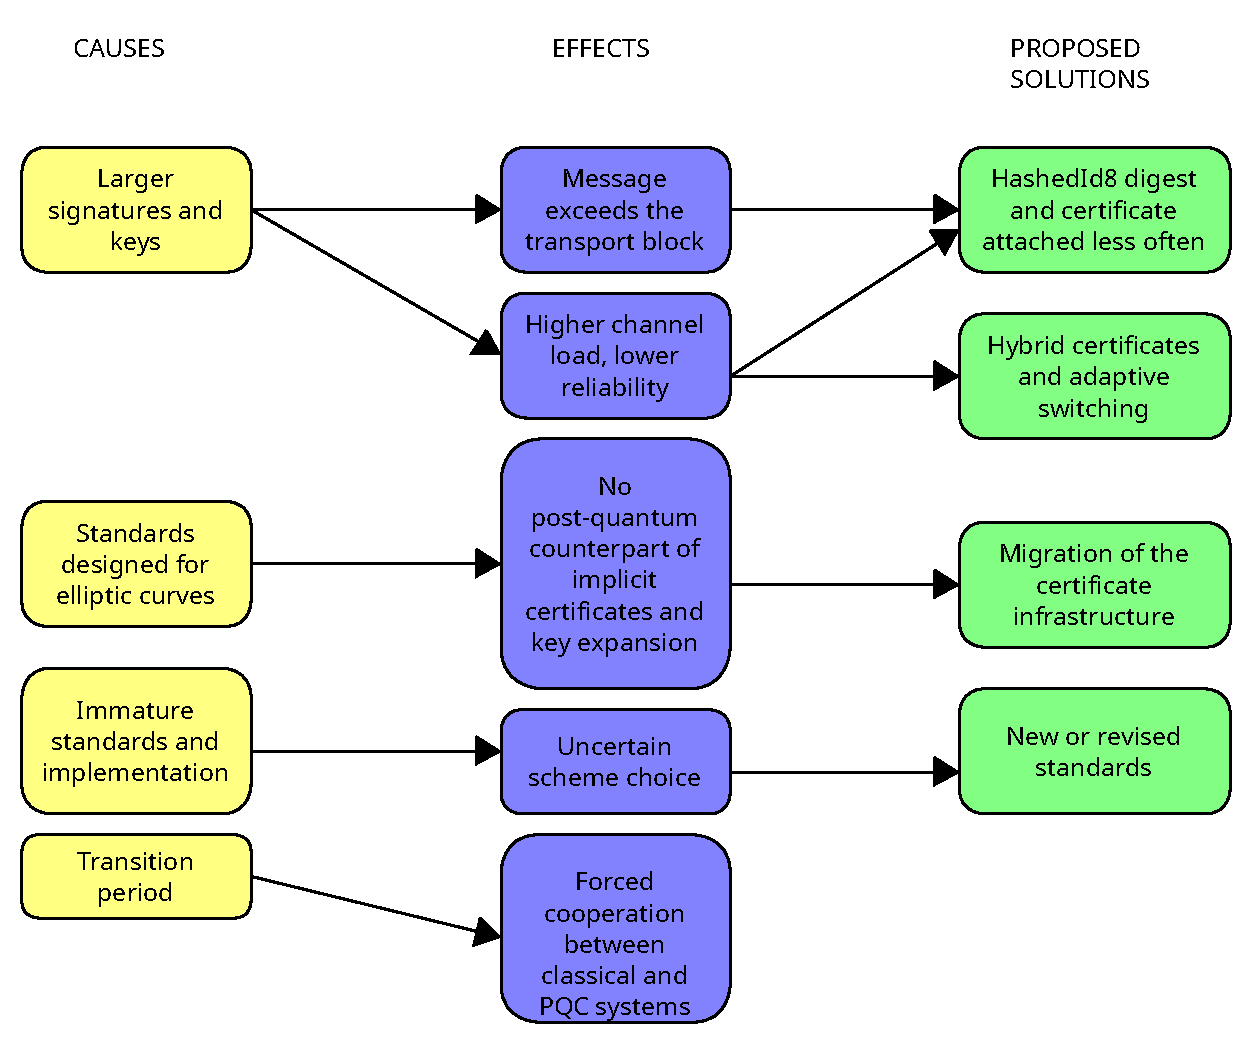
\includegraphics[width=0.7\textwidth]{diagramMIP.pdf}
\caption{Causes of the deployment problems of PQC in V2X, their effects and directions for
improvement. The arrows indicate relation}
\label{fig:map}
\end{figure}

\subsection{Hybrid certificates and adaptive switching}

The NIST transition plan allows hybrid modes in which a post-quantum algorithm is combined with
a classical one~\cite{nistir8547}. The authors of the C-V2X study propose a hybrid ECDSA and
Falcon scheme that would switch between the algorithms depending on channel load, although it
would require changes to IEEE 1609.2 and SAE J3161~\cite{abrar}. The advantage is a smooth
transition, and the disadvantage is a larger message whenever the post-quantum part is used.
Switching to ECDSA alone does not preserve post-quantum signature protection, so a secure
switching policy requires more than a channel-load threshold.

\subsection{Less data in a message}

IEEE 1609.2 already allows the sender to be identified by an 8-byte digest (HashedId8) instead
of the full certificate~\cite{etsi097r1,ieee1609}. If the full certificate is attached less
often, a receiver that already knows it only has to verify the message signature. A rough
calculation based on the sizes in Table~\ref{tab:schemes} shows that the benefit depends on the
scheme. For simplicity, the certificate is counted as the public key only, and the signature of
the issuing authority is ignored. With a naive replacement, where the certificate is attached to
every message, Falcon-512 (signature and key together) has an average overhead of 1\,563\,B. If
the certificate is attached to one message in ten, which corresponds to the current rate of about
one per second at 10\,Hz~\cite{kenney}, and a digest to the others, the overhead falls to about
763\,B, which is 51\,\% less. For ML-DSA-44 (signature and key together 3\,732\,B) it falls to
about 2\,558\,B, only 31\,\% less, because the signature alone makes up almost 65\,\% of that
size.

These percentages are measured against the naive replacement and describe the deliberately
reduced key-and-signature model, not savings for complete transmitted certificates. Because the
one-in-ten schedule equals the current once-per-second practice, the measure does not save
anything beyond that existing schedule; it only prevents the post-quantum overhead from growing
further. Cache misses and delayed certificate availability must be evaluated separately.

\subsection{Migration of the certificate infrastructure}

A central authority issues pseudonym certificates that vehicles rotate to reduce linkability, and
it relies on implicit certificates and key expansion. Both depend on elliptic-curve algebra and
require changes to the provisioning protocol during migration. The back-end process that issues,
rotates and revokes certificates has to be redesigned. The qSCMS proposal describes a
quantum-resistant provisioning process that keeps the SCMS goals (privacy through pseudonyms,
revocation, misbehavior handling) without the elliptic-curve-specific machinery~\cite{barreto},
and the migration framework is described in ETSI TR 103~619~\cite{etsi619}.

\subsection{Similarity to solutions from other fields}

Research on post-quantum X.509 certificates provides a useful comparison: larger credentials add
connection-establishment overhead, although the cited study finds them viable in the protocols it
examines~\cite{kampanakis}. The situation in V2X is stricter, because awareness messages repeat
authentication data over a shared broadcast medium under application-specific deadlines,
including the 100\,ms threshold in the cited C-V2X configuration~\cite{abrar}, so caching, packet
loss and verification have different effects than in one-time website verification. Internet PKI
experience is therefore a starting point; each V2X communication profile needs its own analysis.

\section{Conclusion}
\label{sec:conclusion}

The article examined why deploying post-quantum signatures in V2X requires more than replacing
ECDSA. In the cited C-V2X configuration, the size of the transmitted data is the main
communication constraint, as it limits channel capacity and delivery reliability, while signing,
verification and certificate-processing costs remain platform-dependent. Among the evaluated
candidates, Falcon-512 was the only scheme that satisfied the transport-block constraints of the
considered C-V2X configuration; this finding does not make it the best scheme for all V2X
applications, and its standardization as FN-DSA is still in progress.

The article contributes an overview of the deployment problems supported by the literature, a
comparison of ECDSA, ML-DSA, Falcon and SLH-DSA, an illustrative channel-load calculation, a
certificate-reuse model, and a map that links the causes of the problems to directions for
improvement. What remains open is the measured benefit of improvements for each scheme at
different traffic loads, complete post-quantum certificate formats, secure coexistence during
migration, the finalization of FN-DSA, and validation on representative vehicle hardware. A cited
connected-vehicle exploit study excluded V2X attacks from its scope, so its findings cannot
validate V2X security~\cite{wang}.

\small
\bibliographystyle{plain}
\bibliography{references}

\end{document}
